\documentclass[problem]{mcs}

\begin{pcomments}
  \pcomment{PS_3color_SAT}
  \pcomment{by ARM October 25, 2011}
\end{pcomments}

\pkeywords{
SAT
logical_formula
propositional_logic
logic
proposition
negation
coloring
}

%%%%%%%%%%%%%%%%%%%%%%%%%%%%%%%%%%%%%%%%%%%%%%%%%%%%%%%%%%%%%%%%%%%%%
% Problem starts here
%%%%%%%%%%%%%%%%%%%%%%%%%%%%%%%%%%%%%%%%%%%%%%%%%%%%%%%%%%%%%%%%%%%%%

\begin{problem}
This problem will show that 3-coloring a graph is just as difficult as
finding a satisfying truth assignment for a propositional formula.
The graphs considered will all be taken to have three designated
\emph{color-vertices} connected in a triangle to force them to have
different colors in any coloring of the graph.  The colors assigned to
the color-vertices will be called $T,F$ and $N$.

Suppose $f$ is an $n$-argument truth function.  That is,
\[
f:\set{T,F}^n\to \set{T,F}.
\]
A graph $G$ is called a \emph{3-color-\textit{f}-gate} iff $G$ has $n$
designated \emph{input vertices} and a designated \emph{output
  vertex}, such that

\begin{itemize}

\item $G$ can be 3-colored \emph{only} if its input vertices are
  colored with $T$'s and $F$'s.

\item For every sequence $b_1,b_2,\dots, b_n \in \set{T,F}$, there is
  a 3-coloring of $G$ in which the input vertices $v_1,v_2,\dots,
  v_n\in \vertices{G}$ have the colors $b_1,b_2,\dots, b_n \in
  \set{T,F}$.

\item In any 3-coloring of $G$ where the input vertices
  $v_1,v_2,\dots, v_n\in \vertices{G}$ have colors $b_1,b_2,\dots, b_n
  \in \set{T,F}$, the output vertex has color $f(b_1,b_2,\dots, b_n)$.

\end{itemize}

For example, a 3-color-$\QNOT$-gate consists simply of two adjacent
vertices.  One vertex is designated to be the input vertex, $P$, and
the other is designated to be the output vertex.  Both vertices have
to be constrained so they can only be colored with $T$'s or $F$'s in
any proper 3-coloring.  This constraint can be imposed by making them
adjacent to the color-vertex $N$, as shown in
Figure~\ref{fig:3color-NOT}.

\begin{figure}\inbook{[h]}
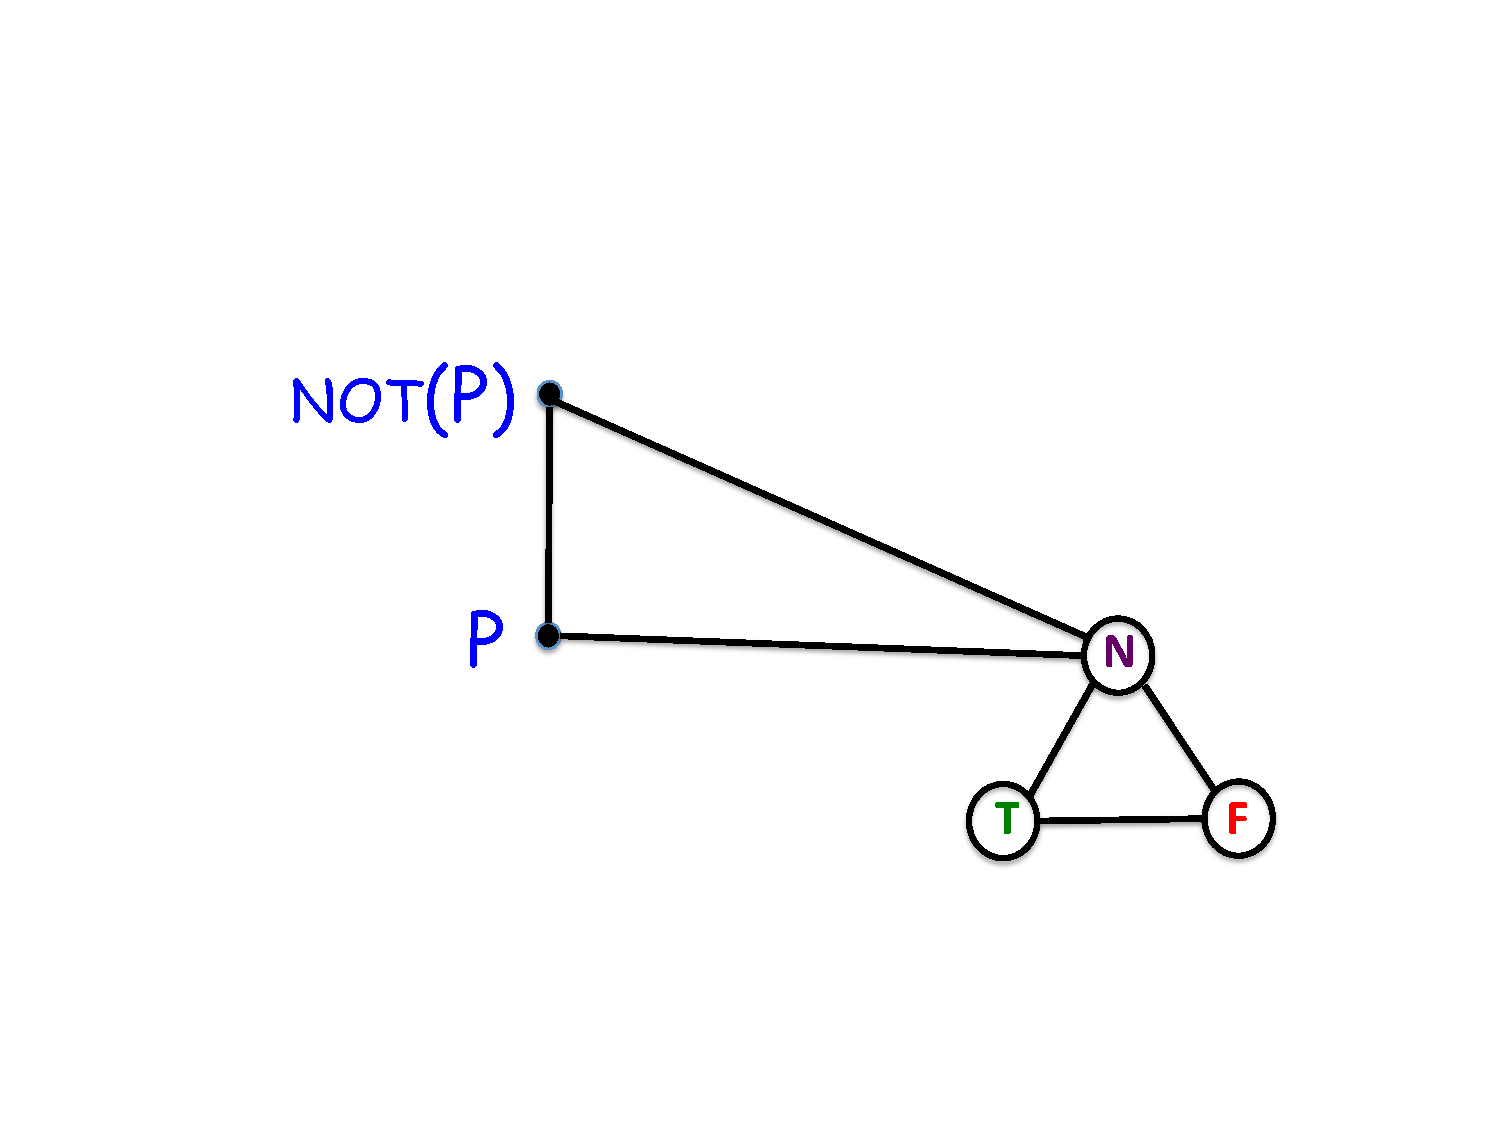
\includegraphics[width=4in]{3color-NOT}
\caption{A 3-coloring $\QNOT$-gate}
\label{fig:3color-NOT}
\end{figure}

\inhandout{\newpage}

\bparts

\ppart Verify that the graph in Figure~\ref{fig:3color-OR} is a
3-color-$\QOR$-gate.  (Color-vertex $F$ and the edges among the
coloring vertices are not shown.  Also not shown are edges from each
of the input vertices $P$ and $Q$ to color-vertex $N$; these edges
constrain $P$ and $Q$ to be colored $T$ or $F$ in any proper
3-coloring.)

\begin{solution}
The diagram is symmetric in $P$ and $Q$, so there only three cases to
consider: $P$ and $Q$ are both colored $T$, both colored $F$, or $P$
and $Q$ are colored differently.  If $P$ and $Q$ are colored
differently, there is only one possible 3-coloring and the output
vertex labelled ``$P$ or $Q$'' is colored $T$.  If $P$ and $Q$ have
the same color, a simple case analysis shows that the output vertex
must also have that color.
\end{solution}

\begin{figure}\inbook{[h]}
\graphic{3color_OR}
\caption{A 3-coloring $\QOR$-gate}
\label{fig:3color-OR}
\end{figure}

\ppart\label{fgateforNOTOR} Let $H$ be an $n$-variable propositional formula that only uses
the operations $\QNOT$ and $\QOR$, and suppose $H$ defines a truth
function $h:\set{T,F}^n\to \set{T,F}$.  Explain a simple way to
construct a graph that is a 3-color-\textit{h}-gate.

\begin{solution}
\TBA{Recursive construction is straightforward}
\end{solution}

\ppart Explain why an efficient procedure for determining if a graph
was 3-colorable would lead to an efficient procedure to solve the
satisfiability problem, SAT.

\hint To determine if propositional formula, $E$, is satisfiable, use
the construction from Problem~\bref{PS_equisatisfiable_3CNF} to find a
formula $J$ using only $\QNOT$ and $\QOR$ such that $J$ is satisfiable
iff $E$ is satisfiable.

\begin{solution}
To determine if a propositional formula, $E$, is satisfiable, use the
construction in Problem~\bref{PS_equisatisfiable_3CNF} to find a 3-CNF
formula, $H$, that is satisfiable iff $E$ is satisfiable.  Then
construct a formula $J$ equivalent to $H$ using DeMorgan's law to
replace the $\QAND$'s in $H$.  Since each application of DeMorgan's
Law replaces a $\QAND$ by two $\QNOT$'s and a $\QOR$, the formula $J$
is easy to construct from $H$ and uses at most three times as many
operations as $H$.  Now build a 3-color-\textit{f}-gate for $J$ using
part~\eqref{fgateforNOTOR}.  Finally, add an edge between the output
vertex of the 3-color-\textit{f}-gate and the $F$-colored vertex; call this
graph $K$.  So $K$ is 3-colorable iff there is a coloring of the input
vertices that makes the output vertex color $T$ which is possible iff
$J$ and hence $H$ and $E$ are satisfiable.  Moreover, the whole
construction of $K$ from $E$ can be done in time proportional to the
the size of $E$, so an efficient procedure to test $K$ for
3-colorability would yield an efficient procedure for to test $E$ for
satisfiability.
\end{solution}

\eparts

\end{problem}

%%%%%%%%%%%%%%%%%%%%%%%%%%%%%%%%%%%%%%%%%%%%%%%%%%%%%%%%%%%%%%%%%%%%%
% Problem ends here
%%%%%%%%%%%%%%%%%%%%%%%%%%%%%%%%%%%%%%%%%%%%%%%%%%%%%%%%%%%%%%%%%%%%%

\endinput
